\section{Hướng dẫn cài đặt và huấn luyện mô hình bằng Google Colab}
\subsection{Kiểm tra môi trường}
Trong giao diện chính của Colab, chọn mục \textbf{Runtime} $\xrightarrow{}$ \textbf{Change runtime type} $\xrightarrow{}$ \textbf{T4 GPU} để chuyển sang chế độ GPU
\begin{figure}[H]
\centering
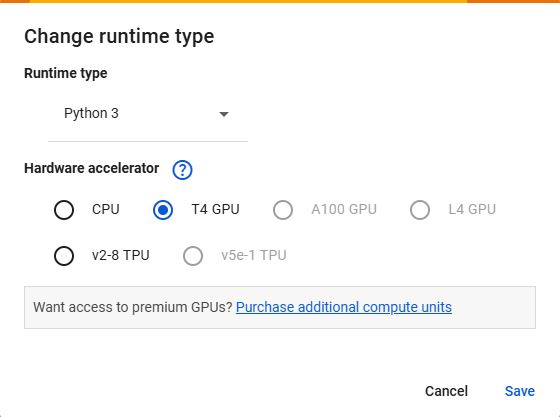
\includegraphics[scale=.4]{img/gpu.JPG}
\caption{Chuyển sang chế độ GPU}
\label{fig:my_label_with_H}
\end{figure}

Có thể kiểm tra lại thông tin GPU bằng câu lệnh
\begin{lstlisting}[language=tex]
!nvidia-smi
\end{lstlisting}

\subsection{Cấp quyền cho Drive}
Cấp quyền để Colab truy cập vào thư mục Drive của người dùng thông qua đoạn mã sau:
\lstinputlisting[language=Python]{code/drive.py}

\subsection{Tải tập tin pretrain}
Tập tin pretrain dùng trong mô hình huấn luyện. Người dùng chỉ cần chọn tập tin pretrain thích hợp và huấn luyện tiếp bộ trọng số có trong tập tin đó để tiết kiệm thời gian thay vì phải huấn luyện mô hình từ con số 0. YOLOv10 cung cấp nhiều tập tin pretrain khác nhau tùy theo mục đích người sử dụng. Dưới đây là đoạn mã ví dụ tải tập tin pretain YOLOv10 - N:
\lstinputlisting[language=Python]{code/pretrain.py}

\subsection{Cài đặt bộ dữ liệu}
\subsubsection{Định dạng cây thư mục dữ liệu}
Đối với các thư mục dữ liệu được sử dụng cho mô hình YOLOv7 trở lên, cây thư mục cần phải có định dạng như sau:
\lstinputlisting[language=tex]{code/tree.tex}
\subsubsection{Cáu trúc tập tin .yaml}
Trong các mô hình YOLOv7 trở lại đây, tập tin .yaml là một tập tin có chức năng hướng dẫn mô hình cần phải trỏ tới thư mục nào để lấy dữ liệu dùng để huấn luyện, đồng thời xác định các lớp nhãn dán có trong mô hình. Cấu trúc một tập tin .yaml gồm có các thành phần như sau:
\begin{itemize}
    \item \textbf{train:} Đường dẫn đến thư mục chứa ảnh trong tập train. Ví dụ: /train/images
    \item \textbf{valid:} Đường dẫn đến thư mục chứa ảnh trong tập valid. Ví dụ: /valid/images
    \item \textbf{train:} Đường dẫn đến thư mục chứa ảnh trong tập test. Ví dụ: /test/images
    \item \textbf{nc:} số lớp nhãn dán
    \item \textbf{names:} danh sách tên các lớp nhãn dán.
\end{itemize}
\subsubsection{Cấu trúc tập tin nhãn dán}
Nội dung của một file nhãn dán trong bộ dữ liệu có thể gồm một số dòng nhất định, trong đó mỗi dòng tượng trưng cho nhãn dán của một đối tượng. Nội dung nhãn dán của một đối tượng có cấu trúc như sau
\begin{lstlisting}[language=tex]
<class_id> <x_center> <y_center> <width> <height>
\end{lstlisting}
Trong đó:
\begin{itemize}
    \item \textbf{class\_id}: ID của lớp đối tượng, là giá trị nguyên bắt đầu từ số 0, phải khớp với thứ tự trong danh sách \textbf{names} trong file .yaml
    \item \textbf{x\_center}: Tọa độ tâm của đối tượng theo chiều ngang.
    \item \textbf{y\_center}: Tọa độ tâm của đối tượng theo chiều dọc.
    \item \textbf{width}: Độ rộng của bounding box.
    \item \textbf{height}: Độ cao của bounding box.
\end{itemize}

Lưu ý: Tên tập tin nhãn dán phải khớp với tên tập tin ảnh. Ngoại trừ \textbf{class\_id}, các giá trị khác của đối tượng phải được chuẩn hóa về khoảng (0, 1) theo tỉ lệ độ dài/rộng của ảnh.

Ví dụ: Một ảnh có kích thước rộng/dài là 800x600 và có thông tin đối tượng như sau:
\begin{itemize}
    \item ID: 0
    \item Tọa độ chưa được chuẩn hóa: (400, 300, 200, 150)
    \item Chuẩn hóa tọa độ tâm: x\_center = 400/800 = 0.5, y\_center = 300/600 = 0.5
    \item Chuẩn hóa kích thước hộp: width = 200/800 = 0.25, height = 150/600 = 0.25
    \item Nhãn dán đã chuẩn hóa: (0, 0.5, 0.5, 0.25, 0.25)
\end{itemize}

\subsection{Huấn luyện mô hình}
Để huấn luyện mô hình, ta chỉ cần gọi thư viện YOLOv10 đẫ tải về trước đó, sau đó gọi lệnh \textbf{!yolo} kèm với đường dẫn chứa tập tin pretrain, tập tin .yaml và một số thông số khác. Dưới đây là ví dụ về đoạn mã huấn luyện mô hình:

\lstinputlisting[language=Python]{code/train.py}

Nếu mô hình được cài đặt và huấn luyện thành công, kết quả trả về sẽ như trong hình minh họa dưới đây.

\begin{figure}[H]
\centering
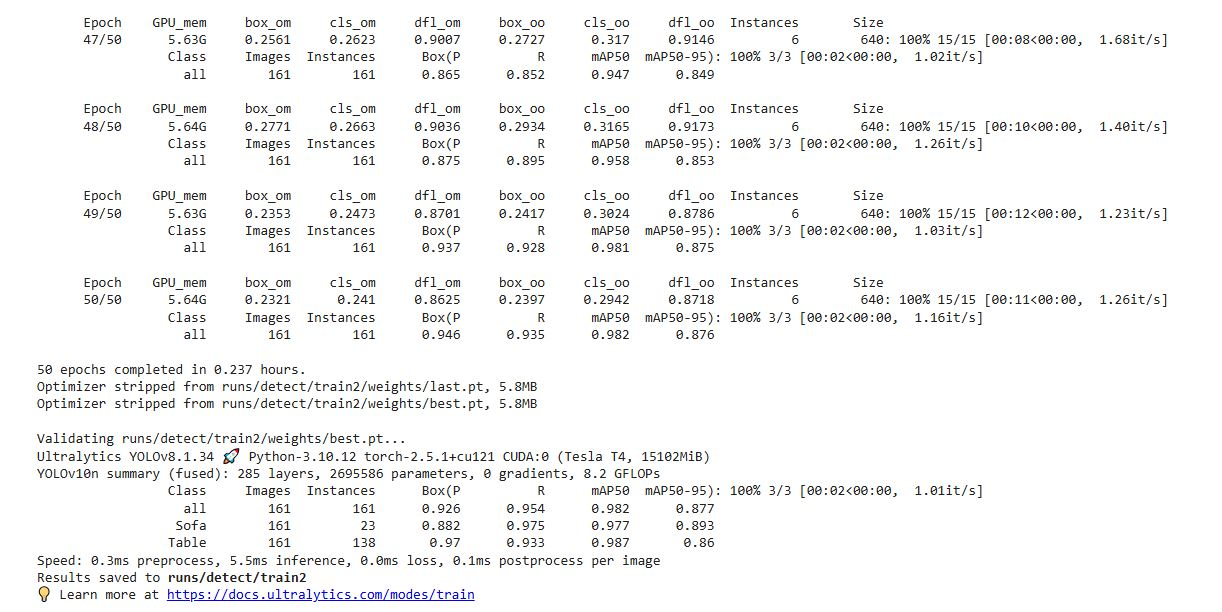
\includegraphics[scale=.5]{img/train.JPG}
\caption{Kết quả sau khi huấn luyện}
\label{fig:my_label_with_H}
\end{figure}